
% Copyright (c) 2015 - 2019 Mario Mlačak, mmlacak@gmail.com
% Published as Public Domain work, under CC0 1.0 Universal Public Domain Dedication. See LICENSING, COPYING files for details.

% Classical Chess -----------------------------------------------------
\chapter*{Classical Chess}
\addcontentsline{toc}{chapter}{Classical Chess}
\label{ch:Classical Chess}

\begin{flushright}
\parbox{0.8\textwidth}{
\emph{A great war leaves the country with three armies -
an army of cripples, an army of mourners, and an army of thieves. \newline
\hspace*{\fill}{\textperiodcentered \textperiodcentered \textperiodcentered \hspace*{0.2em} German proverb} } }
\end{flushright}

\noindent
About Classical Chess is written really everything already, and I have
nothing to add, except to use it as an example on how to read the book.

\clearpage % ..........................................................
% Chessboard, pieces **************************************************

\section*{Chessboard, pieces}
\addcontentsline{toc}{section}{Chessboard, pieces}
\label{sec:Classical Chess/Chessboard, pieces}

The easiest way to introduce readers to the rendering of classical pieces
is to show initial setup chessboard, so here it is:

\noindent
\begin{figure}[!h]
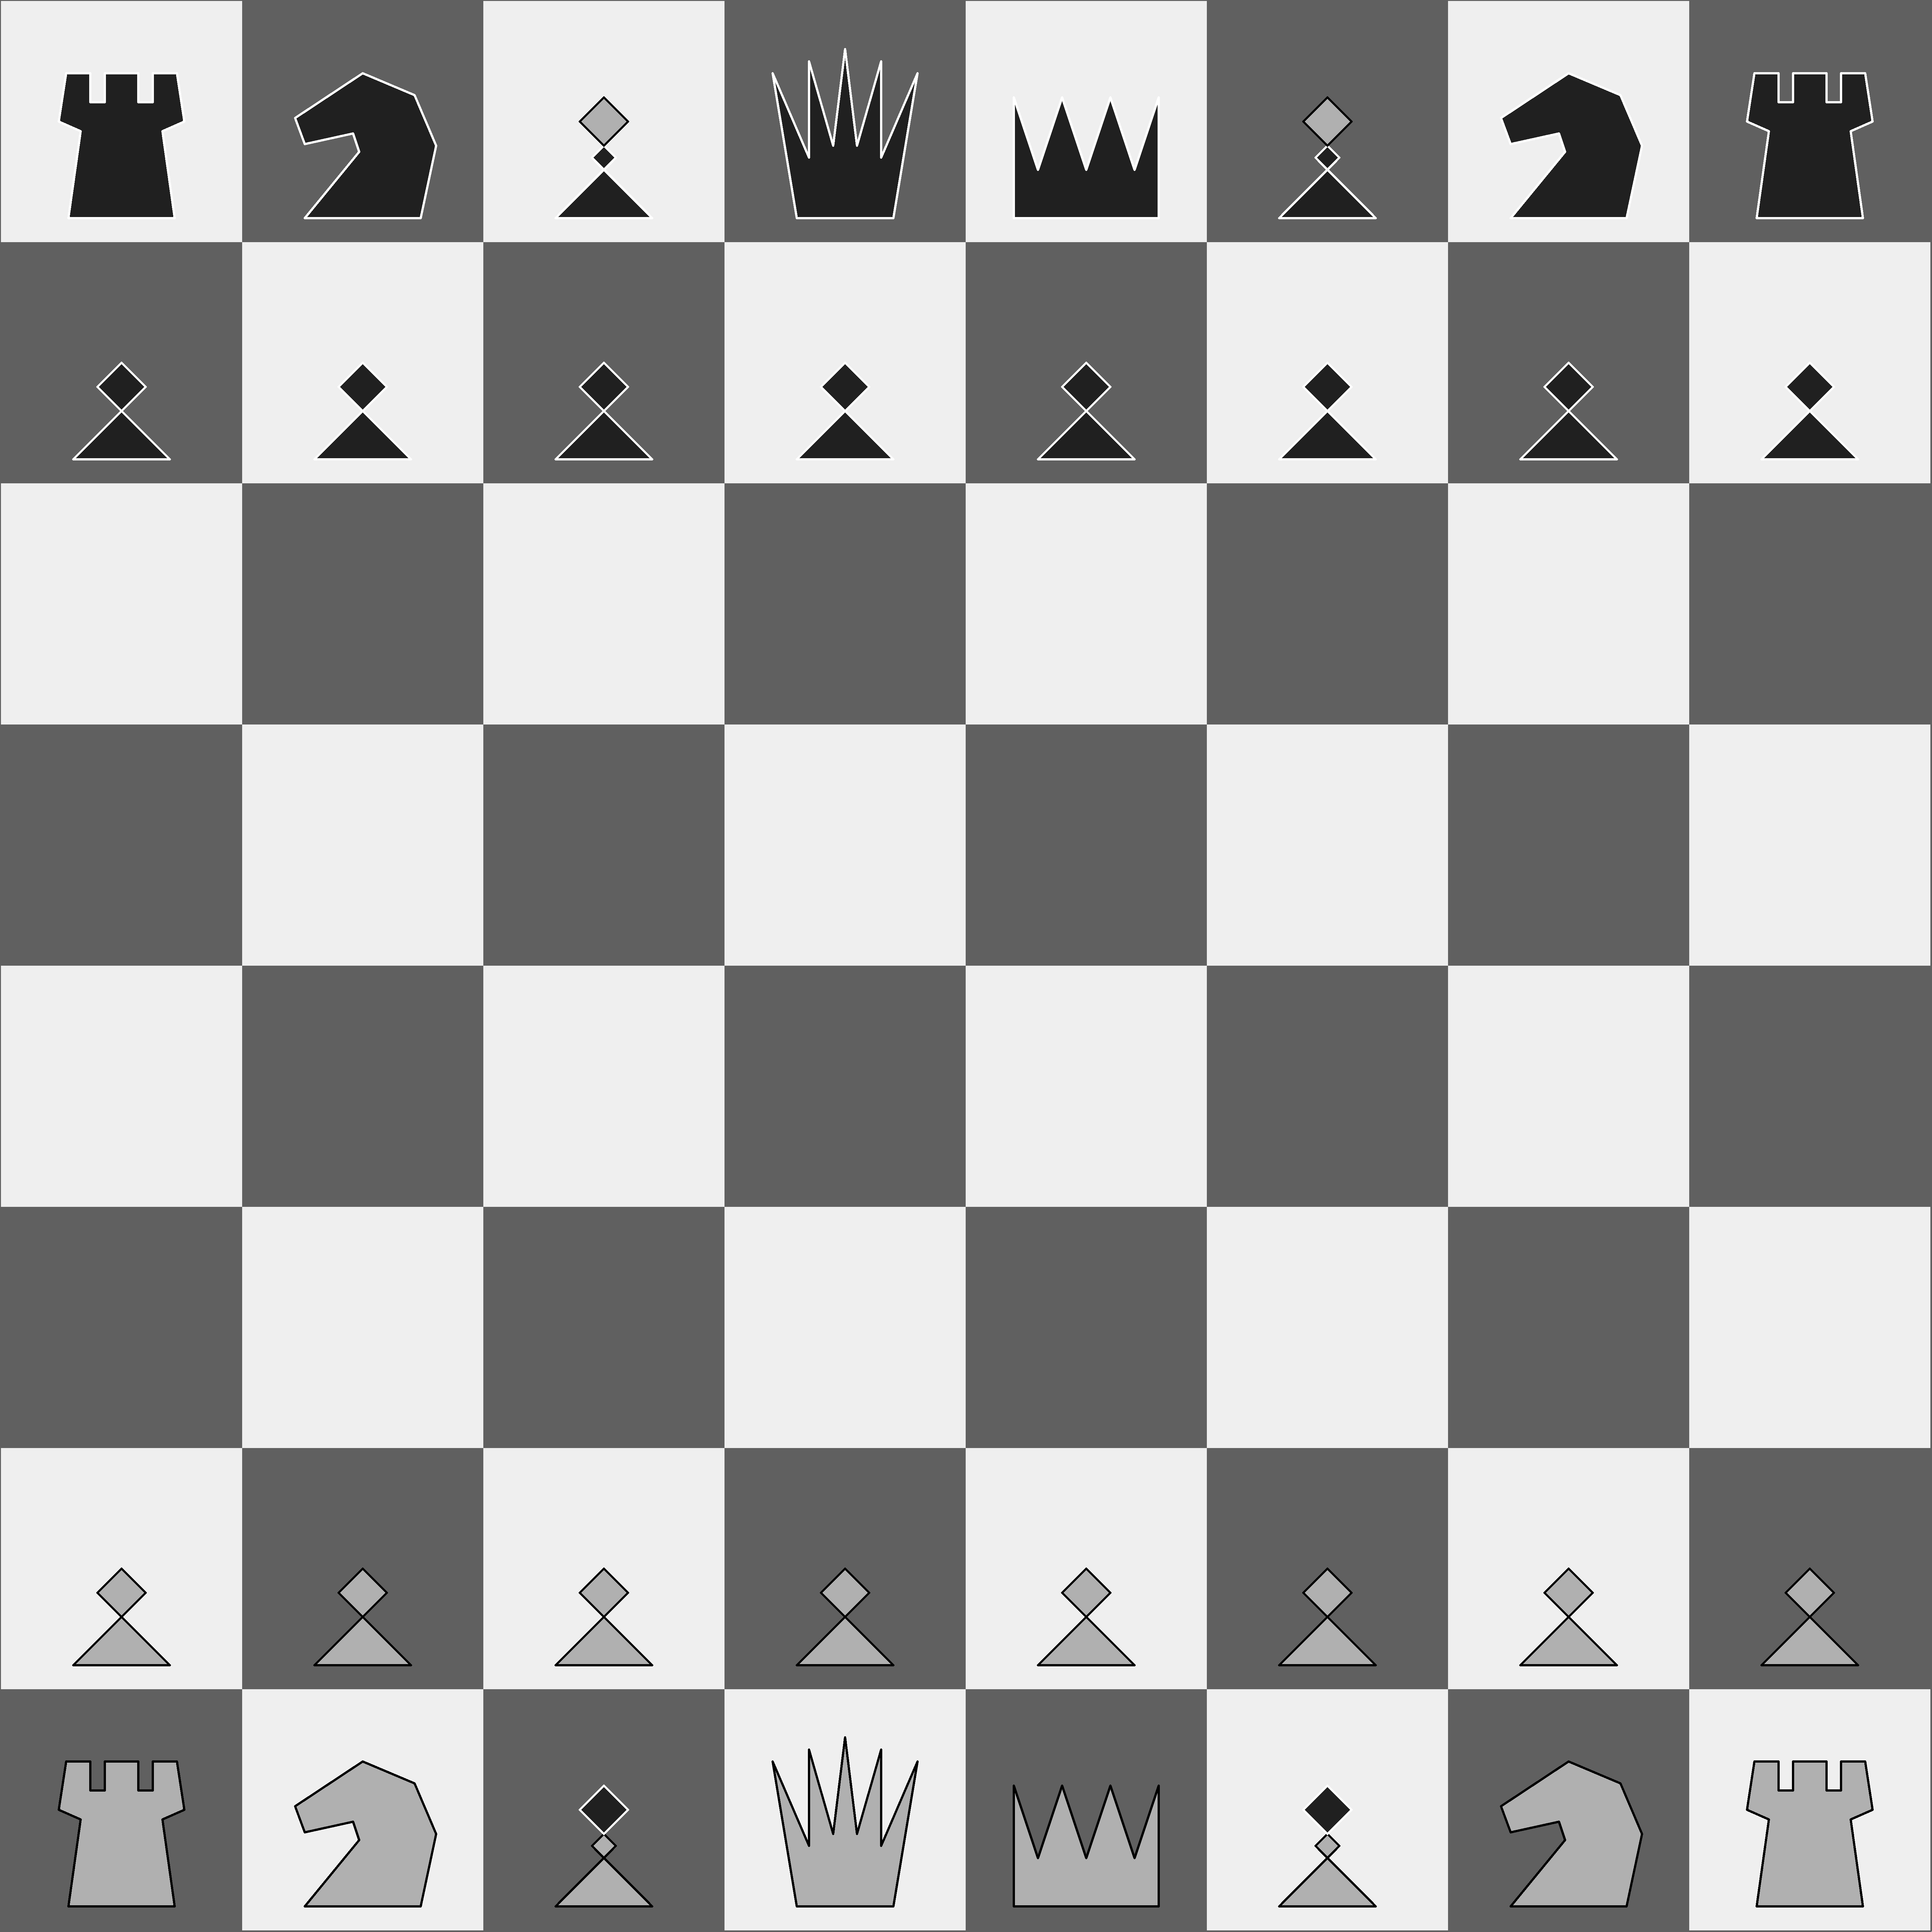
\includegraphics[width=1.0\textwidth, keepaspectratio=true]{boards/02_classical.png}
\caption{Classical Chess, initial setup}
\label{fig:02_classical}
\end{figure}

\noindent
You can compare this with official rendering at \algfmt{FIDE~2.1}.

\clearpage % ..........................................................

\noindent
\TODO :: introduction \newline
\textrightarrow pieces, initial setup \newline
\textrightarrow chessboard sides \newline

% ************************************************** Chessboard, pieces
\clearpage % ..........................................................

\noindent
\textrightarrow basic terminology: turn, move, cycle, figure, ... \newline
\textrightarrow new terminology: rush, steps, step-fields, capture-fields \newline
\textrightarrow conflicting terminology: activating a piece, ply (?) \newline

\noindent
\textrightarrow arrows \& colors \newline
\textrightarrow markers, texts (enumerations vs. labels) \newline
\textrightarrow navigation \newline

\noindent
\textrightarrow context, exceptions \newline

\clearpage % ..........................................................
% ----------------------------------------------------- Classical Chess
